\documentclass[11pt,a4paper]{article}
\usepackage[T1]{fontenc}
\usepackage{amssymb,amsmath}
\usepackage{txfonts}
\usepackage{microtype}

\usepackage[a4paper, total={6in, 10in}]{geometry}

% For figures
\usepackage{graphicx}
\usepackage{subfigure} 
\usepackage[toc,page]{appendix}

% For algorithms
\usepackage{algorithm}
\usepackage{algorithmic}

% For citations
\usepackage{natbib}
\usepackage{hyperref}
\usepackage{url}
\urlstyle{same}
\bibliographystyle{icml2017}
\newcommand{\ubar}[1]{\text{\b{$#1$}}}

\renewenvironment{abstract}
   {
\centerline{\large\bf Abstract}
    \vspace{-0.1in}\begin{quote}}
       {\par\end{quote}\vskip 0.1in}

\begin{document}
\twocolumn[
\title{Natural Computing 2019/2020: Assignment \\ Genetic programming}
\author{School of Informatics, University of Edinburgh \\ s1653529}
\maketitle
]

\begin{abstract} 
\small
With Charles Darwin's publication of The Origin of Species he introduced the basis of a theory that would only gain in influence and importance up until the present time \citep{Darwin}. With the emerging concepts of various algorithms it also found its place in the field of Computer Science, more specifically, it unfolded into the field of Genetic Programming.
This paper puts forward multiple approaches on how genetic programming can be used to generate polynomials that produce as many prime numbers as possible from a given input.
It continues with the presentation of different integer functions for said purpose and finishes with an outlook on alternative applications of genetic algorithms such as neural networks. 
\end{abstract} 
\section*{Introduction}
A number $p$ is a Lucky number of Euler if and only if the prime-generating polynomial $n^2-n+p$ is prime for $n=1, 2, ..., p-1$. It has already been mathematically proven that the only lucky numbers are 2, 3, 5, 11, 17, and 41 \citep{Euler}. This paper does not try to disprove Heegner and Stark \citep{Euler} through extensive exploration as this would be a waste of energy and time. This paper attempts to explore various polynomials, later more general function-combinations and their ability to produce primes.
\\ \\
Genetic Programming starts out with a population of computer programs. These programs can be chosen at random, initialised by another algorithm or initialised according to a specific distribution. It then proceeds to evaluate all programs in the population. The program evaluations are done through a so called fitness function. Subsequently, the most useful programs are kept from the population while the less useful programs are discarded. This step will be referred to as the selection process. From this reduced population, a subset is selected with the aim to recombine the programs within and replenish the reduced population by a certain amount. This process is denoted as the crossover phase. It then continues to iteratively apply these last two steps to the population until the predefined terminal condition is met.
\\ \\
This paper starts out with an attempt to reproduce the polynomial $x^2+x+41$ with a Genetic Algorithm. The results will serve as a baseline model. Since it is a lot faster than the GP-algorithm it will help to establish reasonable bounds for our parameters. The parameters are chosen is such a way that they are comparable. The GA offers a sensible starting point. Followed by that, it will present an implementation of a Genetic Program and the experiments that were carried out with it. Lastly, it will combine the GP and Simulated Annealing to reduce the number of initially useless programs and offers an outlook on the applications of GPs.
\section*{Basic Concept}
\subsection*{Fitness function}
For the evaluation of the GA and the GP a function $f$ is utilized that combines three fitness functions by adding their scores. The scores are not weighted. The first fitness function returns the number of primes that were produced by the polynomial on a given input interval. The second fitness function returns the maximal number of consecutively produced primes on the given input interval $X = [0, 200)$. The last fitness function only returns the number of primes that are consecutively produced when starting at the lower bound of the input interval. A polynomial $p$ is evaluated via
\begin{align*}
f(p) = &f_1(p)+f_2(p)+f_3(p) \\
f_1(p) = &|\{p(x_i) \in \mathbb{P} \; | \; x_i \in X \}| \\
f_2(p) = &\max_{x_k \in X}|\{x_{i} \; | \; x_{i}, x_{i-1}, ..., x_k \in X, \\ & p(x_{i}), p(x_{i-1}), ..., p(x_k) \in \mathbb{P} \}| \\
f_3(p) = &|\{x_{i} \; | \; x_{i}, x_{i-1}, ..., x_0 \in X, \\ & p(x_{i}), p(x_{i-1}), ..., p(x_0) \in \mathbb{P} \}|,
\end{align*}
where $\mathbb{P}$ denotes the set of prime numbers.
\subsection*{Populations}
The GA/GP starts with a population of polynomials of a given size. Multiple populations can be chosen to evolve in parallel. The populations merge whenever a critical, predefined population size is reached. The GA/GP iteratively goes through the selection process followed by the repleshing of the population. The GA/GP stops and returns its result as soon as the population size stagnates.
\subsection*{Selection}
In the selection process the polynomials with a fitness score above the population's fitness mean $f_{\mu}$ remain in the population. The rest of the population is discarded. The selection process redefines a population $P_r$ via
\begin{align*}
P_r \leftarrow \{p \in P_r \; | \; f(p) \geq f_{\mu}\}
\end{align*}
\subsection*{Replenishment}
Subsequently, the number of the discarded polynomials $P_d$ is determined. The remaining polynomials $P_r$ are then taken and recombined in the crossover phase. The population is replenished by an amount $\eta \cdot |P_d|$ where $\eta$ is the replenishing-rate also denoted as the birth-rate here. We summarize the replenshing phase via
\begin{align*}
P_r = P_r \cup \; Crossover \left(\bigcup_{i=1}^{\eta \cdot |P_d|} p_i, \bigcup_{j=1}^{\eta \cdot |P_d|} p_j\right), \\ \; p_i, p_j \sim D(\epsilon),
\end{align*}
where $\epsilon \propto 0.1 \cdot |P_r|$ and avoids zero-divisions. The crossover-function recombines features of the polynomials from the two given input sets. This will be explained in later sections. $D(\epsilon)$ is a probability distribution over $P_r$ following 
\[ 
d(p|\epsilon)= \frac{f(p)+\epsilon}{\sum_{p_k \in P_r} (f(p_k) + \epsilon}.
\]
\section*{Baseline}
\subsection*{Concept}
As mentioned before, a GA was chosen to represent our baseline for comparisons. \\
The chromosome of a polynomial in the implemented GA consists of its coefficients incorporated into an array of the size of its order. The bound for the coefficients is predefined. The bound of the order of the polynomial is also set beforehand and can be regarded as an additional feature in the polynomial's chromosome. The coefficients and the order are initialised via a uniform distribution over the given bounds. Firstly, the order is determined. The coefficients follow. \\
The {\bf crossover-function} takes one polynomial from the first input set and combines it with another polynomial of the second input set with a coinciding index. Hence, each pair produces one offspring polynomial. It is very much possible that a polynomial is recombined with a copy of itself. The recombination works through extending both coefficient arrays with zeros to a length that goes up to the order constraint. The new polynomial is then formed by selecting either of the respective coefficients from the two arrays factor-wise. \\
The resulting array is then passed through mutation function with a with a predefined mutation probability. The mutation function then selects a coefficient from the zero-extended resulting array and substitutes it by a new coefficient value selected from the uniform distribution over the coefficient bounds. The leading zeros are then discarded.
\subsection*{Setting the Baseline}
For $x^2+x+41$ we record a fitness score of 236, producing 156 primes on the input interval. Evidently, the starting streak is the longest streak with a length of 40 consecutively produced primes. After several trials the GA that reproduced the polynomial in a reliable manner had one population of 5000 polynomials, a birth-rate of 0.7, a mutation-rate of 0.1, a coefficient bounding of $[1, 41]$, and an order restriction of at most degree 2 (Figure \ref{fig:baseline}). It converged after just under 35 generations (other trials managed to converge close to 25). One can observe that there was a rather big oscillation in fitness at generation 17 and 29. Before generation 17, one can assume that it was stuck in a local maximum as it also seemed to stagnate. The rather high mutation-rate could have contributed to it proceeding to improve.
\section*{Genetic Program Implementation}
\subsection*{Concept}
The chromosome of the function to be produced by the GP is represented by a syntax tree (see Figure \ref{fig:syntax_tree}). The leaf-nodes are either terminal or non-terminal. Terminals are simply integers while non-terminals are variable. The internal nodes form sets of nested functions. The set of functions to choose from can be passed in as an argument of the population. Previously established coefficient bounds are also applied on the terminals here. The order bound is now implicitly given by limiting the depth of the tree. A tree is initialised by creating internal nodes down to the depth-limit. The function is chosen randomly from the set of passsed in functions. The leaves are then randomly filled by either terminal or non-terminal nodes. \\
The {\bf crossover-function} takes one tree from the first input set and combines it with another tree from the second input set with coinciding index. Each tree pair produces one offspring tree. Both input tree are then dissected. In the first input set we select the nodes of all trees that are above half the depth limit and add them to a breeder set. In the second input set we select the nodes of all trees that are below half the depth limit and add them to another breeder set. Any of the child nodes of the nodes in the first breeder set can then be substituted by any node, including its child nodes, of the second breeder set as long as their indices coincide. This is done in a purely random manner again. \\
A node of the second breeder set has a chance to be substituted by a randomly generated tree of half the depth of the depth limit. The probability of the substitution is determined by the mutation-rate parameter.
\subsection*{Experiments}
Using the same parameters as with the GA, i.e. a depth limit of 3, we also manage to reproduce the polynomial $x^2+x+41$. It took around 30 generations longer to converge. Though, the GP produced the polynomial a lot more reliable than the GA. The average fitness oscillated more heavily than with the baseline. Suprisingly, it did not take longer because $x^2+x+41$ did not appear in the population until the very end. $x^2+x+41$ actually, most likely already appeared in the 2nd generation when using the GP. The population utilizing the GA needed 17 generations for that. The GP also seems to provide a greater diversity in the top performing polynomials (see Figure \ref{fig:tree_ga_comparison_2} and Figure \ref{fig:tree_ga_comparison}). Figure \ref{fig:tree_phases} shows the effects of the two different phases on the average fitness throughout the generations. The differences become more severe in the final generations, suggesting that the fitness deviation from the mean increases.\\
Expanding the coefficient bounds from $[1, 41]$ to $[-61, 61]$ and increasing the depth limit from 3 to 5 effectively increases the search space. The consequences are quite evident to observe. While the converging time did not increase, it did not perform well. With a final fitness score of 145, it settled on a significantly worse polynomial than $x^2+x+41$ (see Figure \ref{fig:custom_tree_1}). \\
One could counter this by simply increasing the population size. Instead of following that approach, one can introduce multiple populations and evolve them in parallel. In the next experiment three populations developed in parallel until the number of polynomials in the first population dropped to under 40\% of its original size. This slightly increased the final fitness score to 154 (see Figure \ref{fig:custom_tree_2}).
\\
The next experiment attempts to offer a look into the direct influence of the mutation-rate onto the performance. The low mutation-rate seems to do well and actually questions the previous assumption that the mutation rate was responsible for the oscillations. Additionally, the low mutation-rate seems to have had an effect on the $f_2$- and $f_3$-scores. The population with the low mutation-rate had a prime streak that was longer by 24 consecutive inputs. The fitness comparison graph (Figure \ref{fig:mutation_tree_2}) suggests that the crossover could not lead to major improvements due to very likely, subsequent mutation. For a comparison of the average fitness, see Figure \ref{fig:mutation_tree}. \\
Up to this point the GP only made use of two functions, namely addition and multiplication. Three functions that are excellent candidates for expanding the set of possible functions are $g_1(a, b)=max(a,b)$, $g_2(a, b)=min(a,b)$ and $g_3(a, b)= a \; \mod \; b$. The mod-function defines taking something mod 0 as 0 here. Only using these three functions with previous parameters decreased the final score to 49. The average fitness oscillated substantially more. 
\\
Using the function set [addition, multiplication, maximum, mod] with a 40\% chance for the maximum function (20\% for the other functions respectively) delivered unexpected results. Not only did the final function reach the previous maximum score of 236, with 40 consecutive primes starting at 0, with a total of 156 primes. It managed to do this in just 25 generations, therefore, being even faster than the GA. It should also be noted that the search space was substantially larger than when the GA ran. The final tree most likely appeared first in generation 11. The average fitness oscillated less heavily (see Figure \ref{fig:extension_function_1}). When considering numpy's mod function the tree actually collapses to $x^2 + x + 41$ (see Figure \ref{fig:extension_function_2}). Using the function set [addition, multiplication, maximum, minimum, mod] delivered similar results in 40 generations.
\subsection*{Experiments with Simulated Annealing}
We can incorporate local search methods into the GP to quickly determine the terminal values of the tree. Using Simulated Annealing (Algorithm \ref{alg:SimAnn}) on the terminal values of a random tree with a fitness score of 0 improved to 8 with 1000 iterations a temperature of 100000 and a temperature change of 0.98. When combined with the actual GP with 700 iterations a temperature of 70000 and a temperature change of 0.98 the GP converged within 26 generations. That's a reduction by more than half compared to the GP presented in Figure \ref{fig:tree_ga_comparison}. The final polynomial most likely already appeared in generation 3 (see Figure \ref{fig:simAnn_1}). The effect of the local search can be observed in Figure \ref{fig:simAnn_2} and is essentially depicted by the height difference between a green bar and the respective next blue bar.
\section*{Outlook}
\bibliography{example-refs}
\begin{appendices}
\subsection*{Baseline}
\begin{figure}[h]
\centering
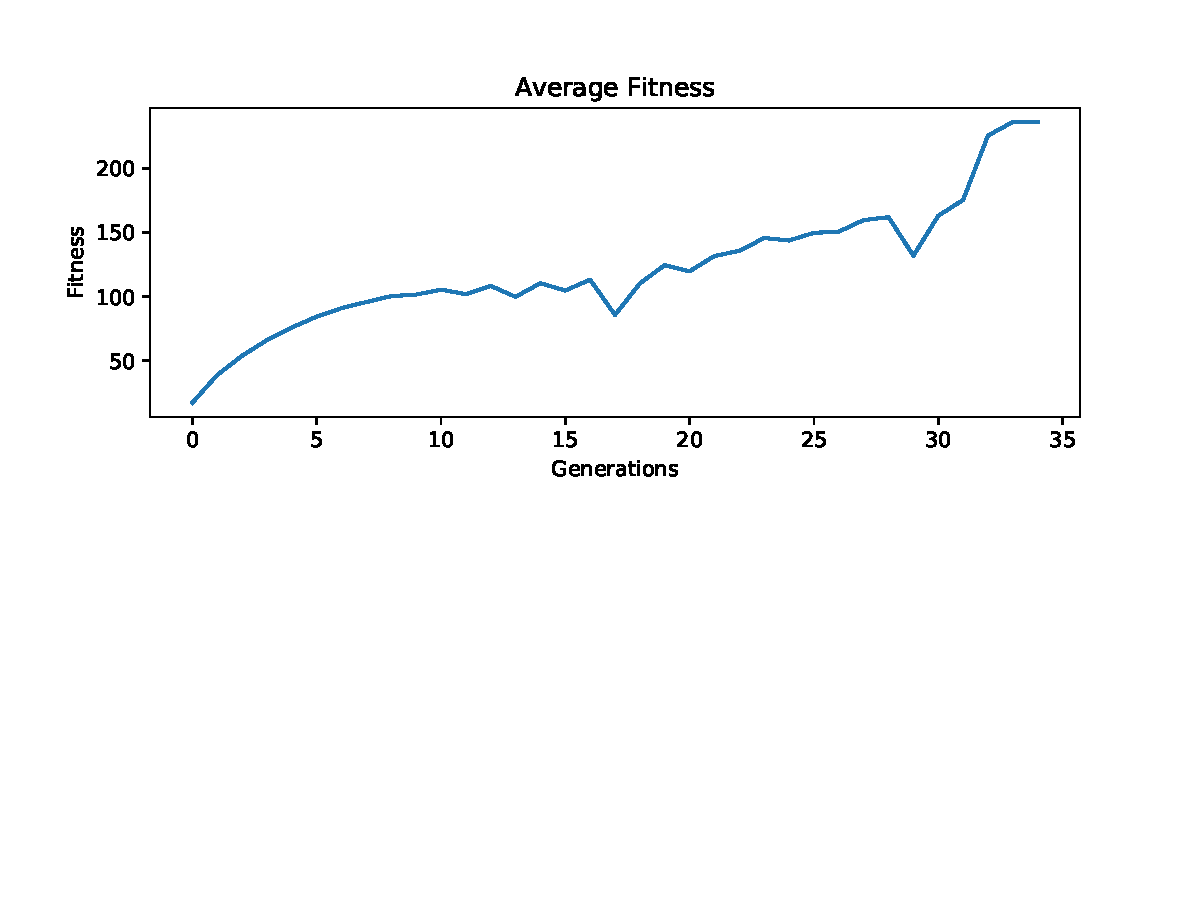
\includegraphics[scale=0.41, clip, trim=0.5cm 7.2cm 0.5cm 0.7cm]{../../NatComputingCW/reproduction_ga.pdf} 
\caption{Average fitness of the GA Baseline over its generations}
\label{fig:baseline}
\end{figure}

\subsection*{Genetic Program Implementation}
\begin{figure}[h]
\centering
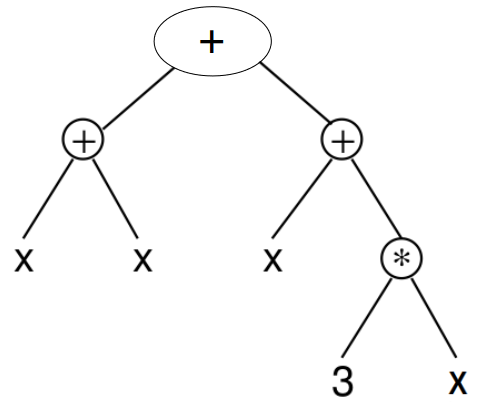
\includegraphics[scale=0.25]{../../NatComputingCW/GP_tree.png} 
\caption{Tree-structure of a polynomial produced by a GP, i.e. $6x$}
\label{fig:syntax_tree}
\end{figure}

\begin{figure}[h]
\centering
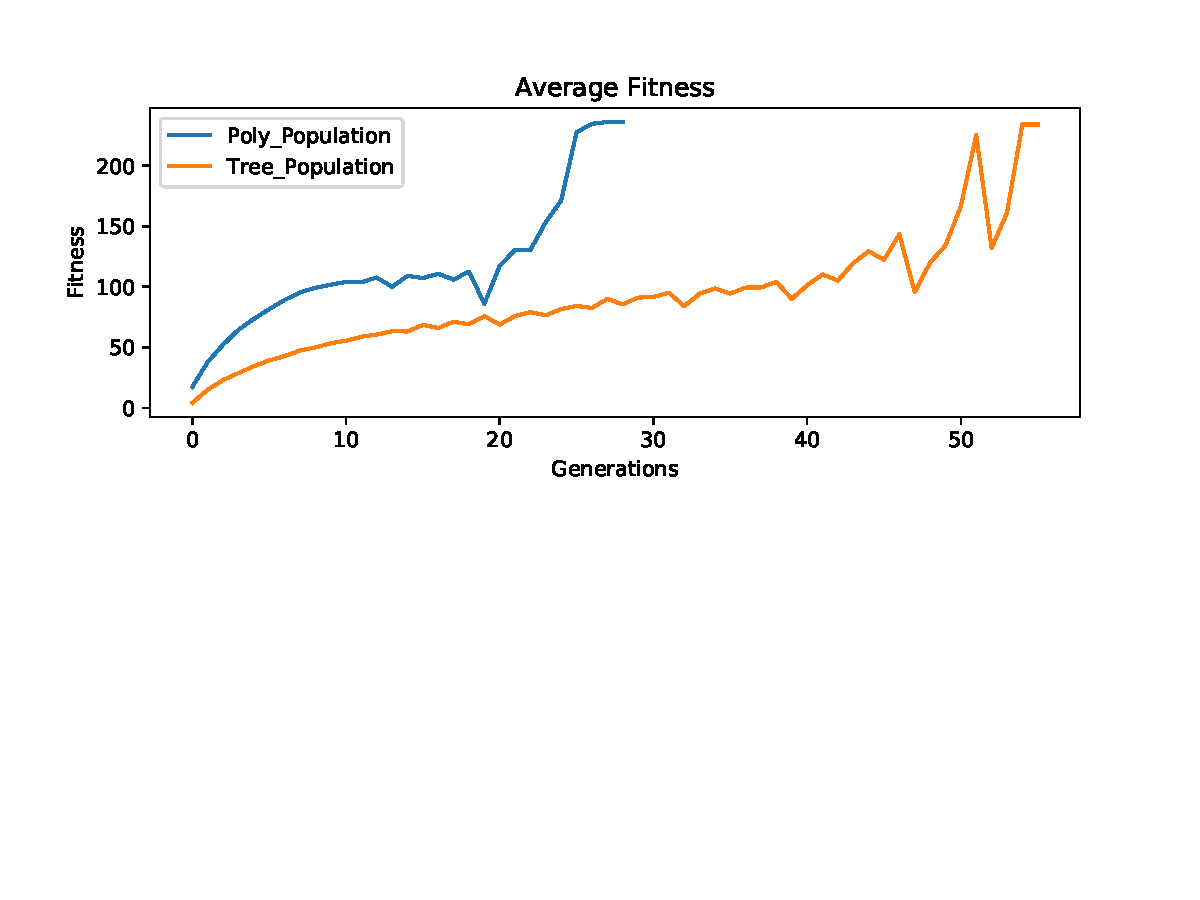
\includegraphics[scale=0.41, clip, trim=0.5cm 7.2cm 0.5cm 0.7cm]{../../NatComputingCW/tree_ga_comparison.pdf} 
\caption{Comparison of the average fitness of the baseline/GA (Poly Population) and the GP (Tree Population) throughout the generations}
\label{fig:tree_ga_comparison}
\end{figure}

\begin{figure}[h]
\centering
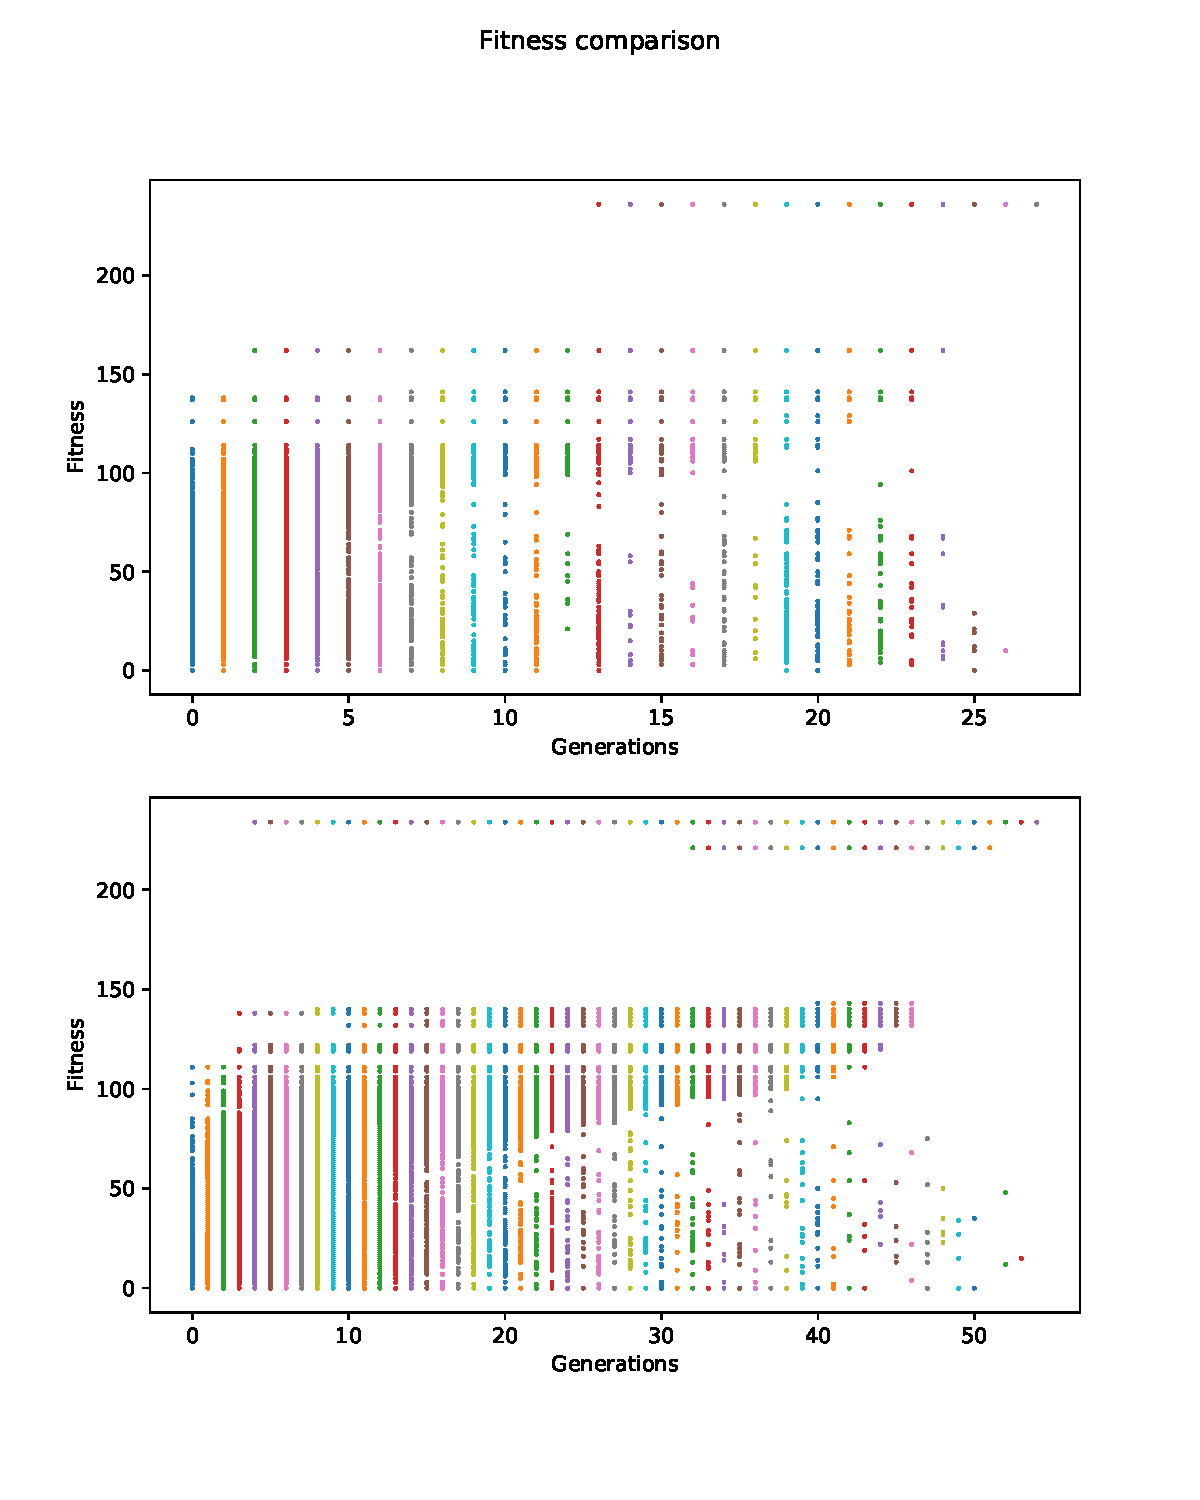
\includegraphics[scale=0.41, clip, trim=0.5cm 2.2cm 0.5cm 0.5cm]{../../NatComputingCW/tree_ga_2_comparison.pdf} 
\caption{Comparison of the fitness of the baseline/GA (top) and the GP (bottom) polynomials throughout the generations, each polynomial fitness score recorded}
\label{fig:tree_ga_comparison_2}
\end{figure}

\begin{figure}[h]
\centering
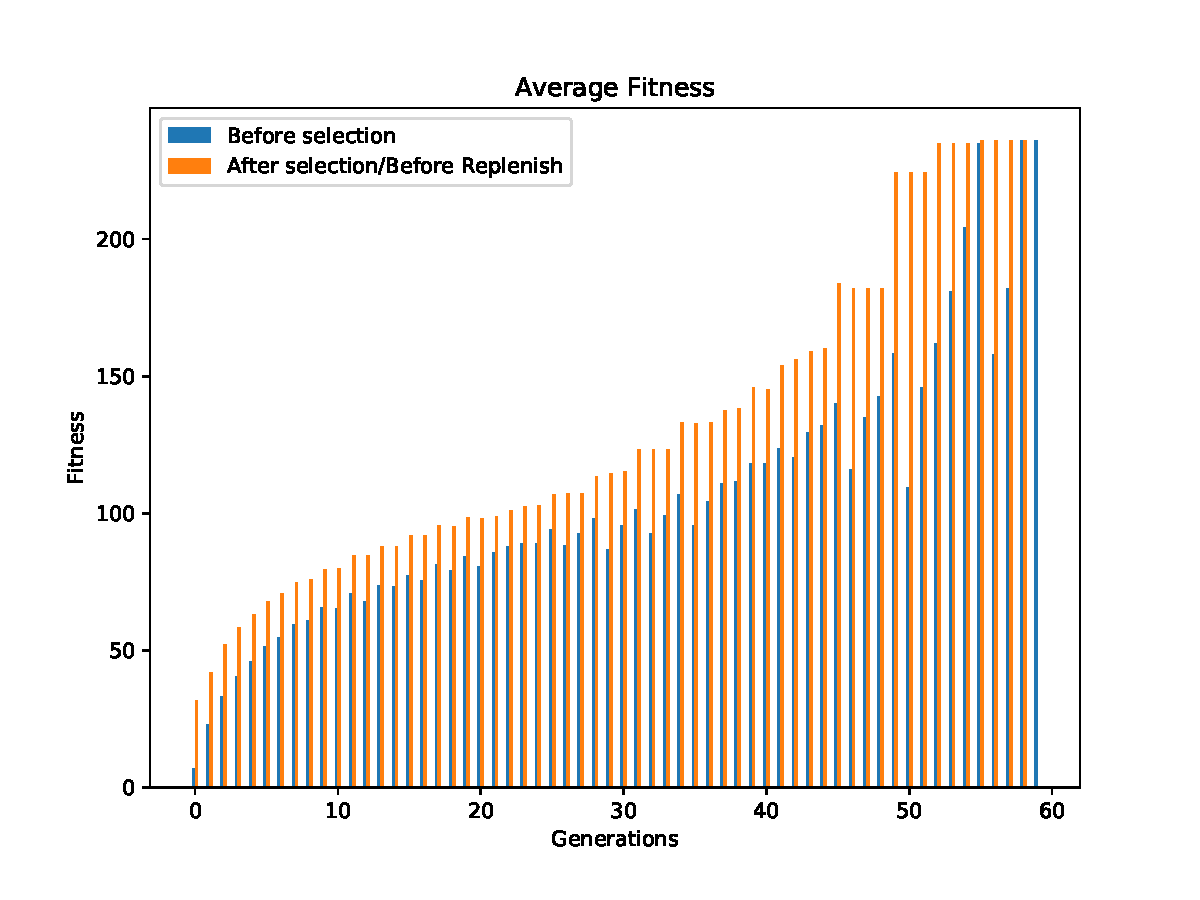
\includegraphics[scale=0.41, clip, trim=0.5cm 0.9cm 0.5cm 1.2cm]{../../NatComputingCW/tree_phases.pdf} 
\caption{Comparison of the average fitness in selection phase and replenishing phase throughout the generations}
\label{fig:tree_phases}
\end{figure}

\begin{figure}[h]
\centering
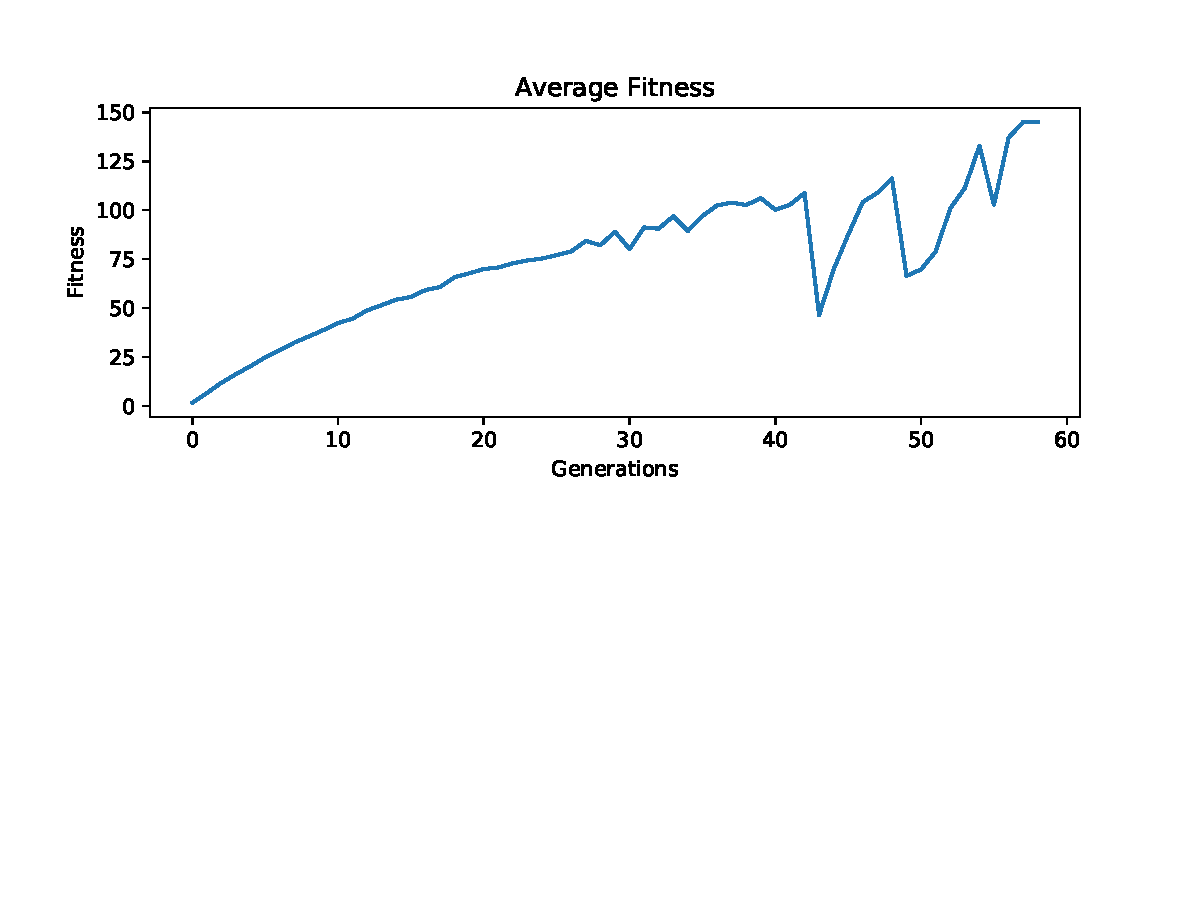
\includegraphics[scale=0.41, clip, trim=0.5cm 7.2cm 0.5cm 0.7cm]{../../NatComputingCW/custom_tree_1.pdf} 
\caption{Average fitness throughout the generations with increased search space, i.e. coefficient bounds $[-61, 61]$, depth limit 5 (number of populations 1, population size 5000, birth-rate 0.7, mutation-rate 0.1)}
\label{fig:custom_tree_1}
\end{figure}

\begin{figure}[h]
\centering
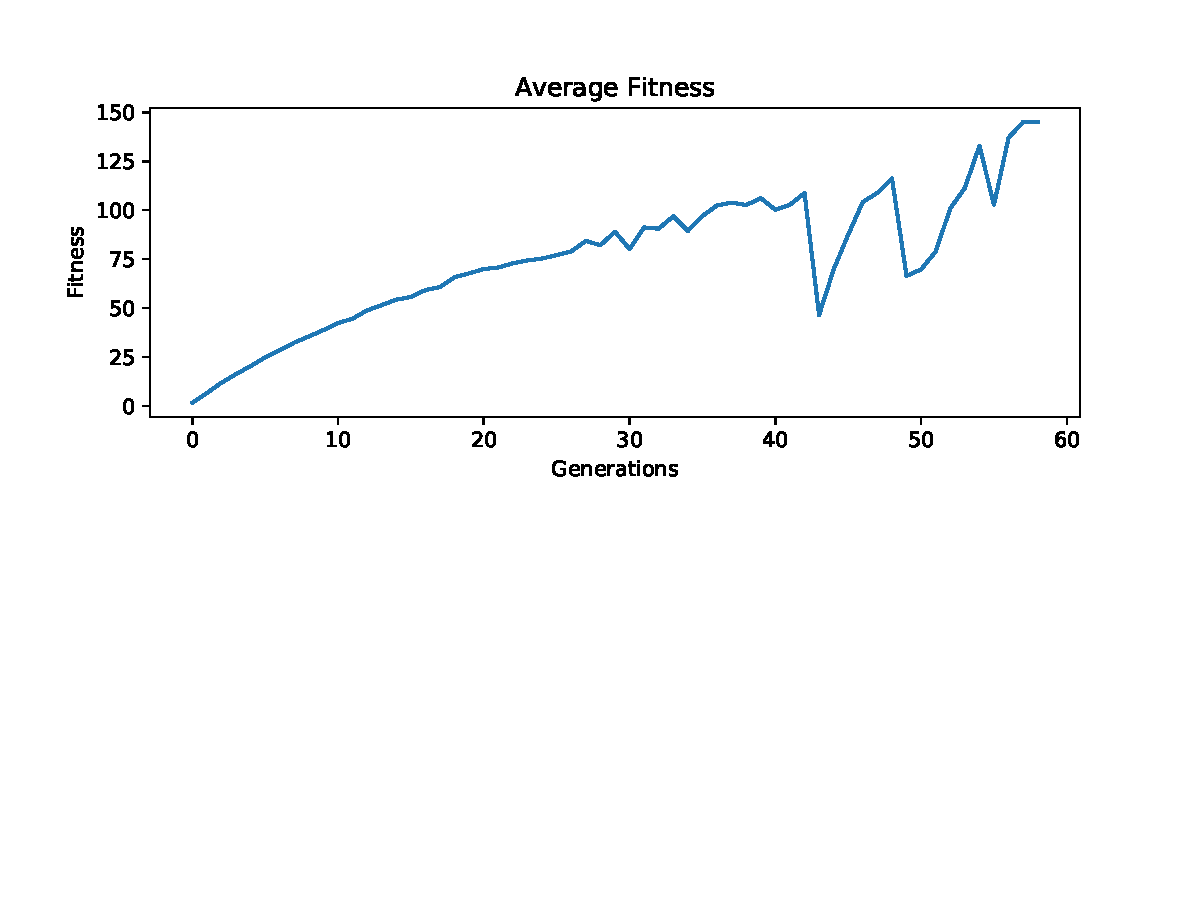
\includegraphics[scale=0.41, clip, trim=0.5cm 7.2cm 0.5cm 0.7cm]{../../NatComputingCW/custom_tree_1.pdf} 
\caption{Average fitness throughout the generations with multiple populations, i.e. 3 (coefficient bounds $[-61, 61]$, depth limit 5, number of populations 1, population size 5000, birth-rate 0.7, mutation-rate 0.1)}
\label{fig:custom_tree_2}
\end{figure}

\begin{figure}[h]
\centering
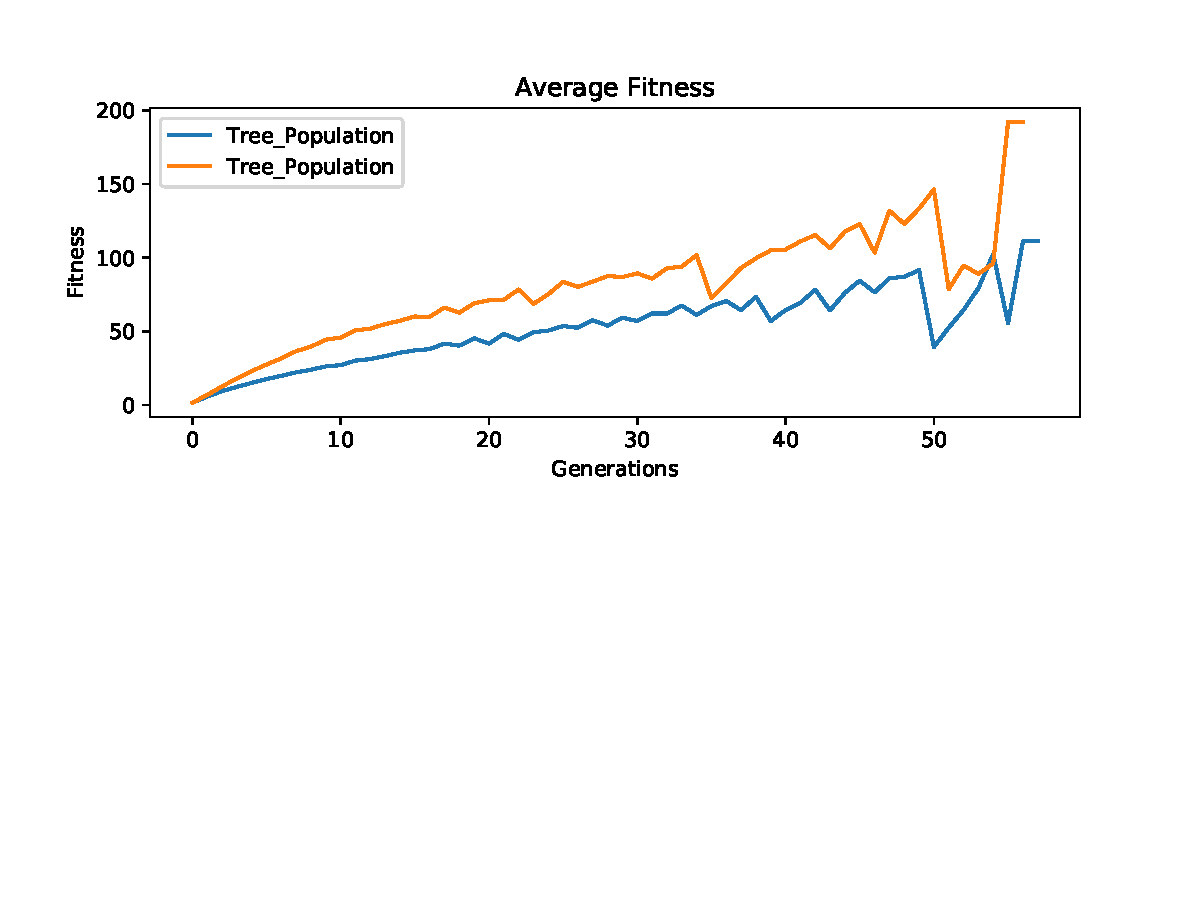
\includegraphics[scale=0.41, clip, trim=0.5cm 7.2cm 0.5cm 0.7cm]{../../NatComputingCW/tree_mutation_comparison.pdf} 
\caption{Average fitness of the GP throughout the generations with decreased mutation-rate (0.01, orange) and increased mutation-rate (0.5, blue) (number of populations 1, coefficient bounds $[-61, 61]$, depth limit 5, population size 5000, birth-rate 0.7)}
\label{fig:mutation_tree}
\end{figure}

\begin{figure}[h]
\centering
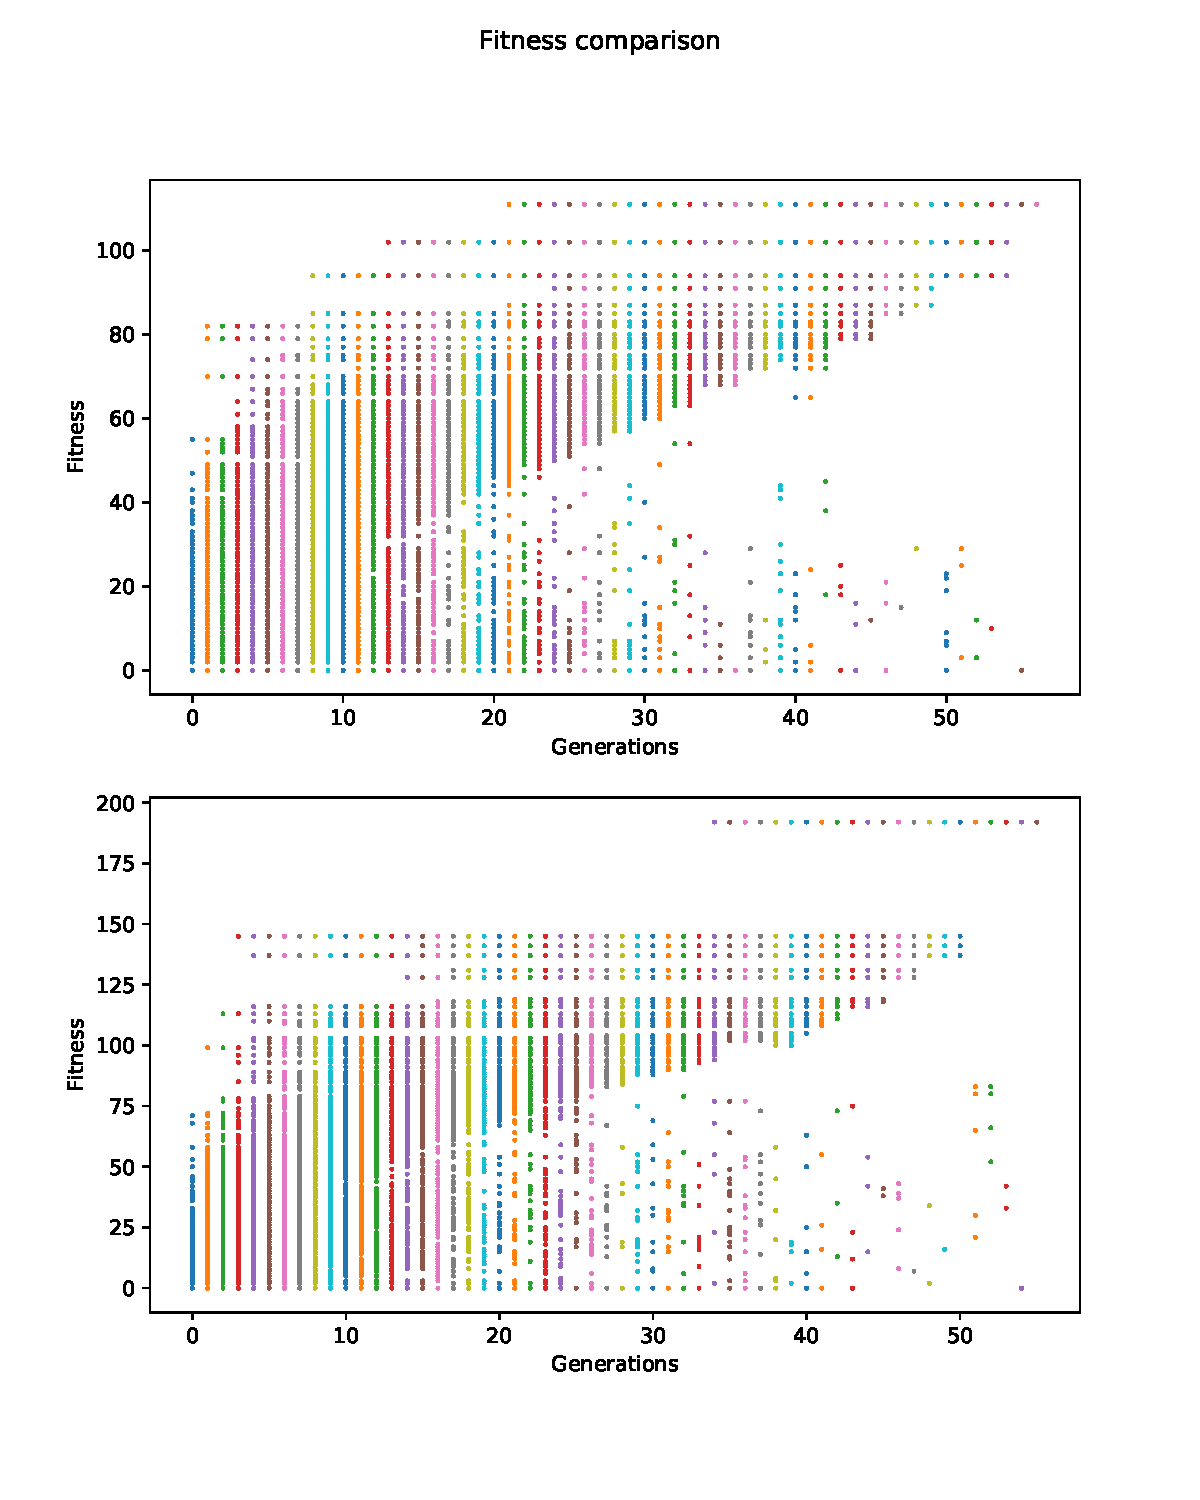
\includegraphics[scale=0.41, clip, trim=0.5cm 2.2cm 0.5cm 0.5cm]{../../NatComputingCW/tree_mutation_2_comparison.pdf} 
\caption{Fitness of the GP throughout the generations with decreased mutation-rate (0.01, top) and increased mutation-rate (0.5, bottom) (number of populations 1, coefficient bounds $[-61, 61]$, depth limit 5, population size 5000, birth-rate 0.7)}
\label{fig:mutation_tree_2}
\end{figure}

\begin{figure}[h]
\centering
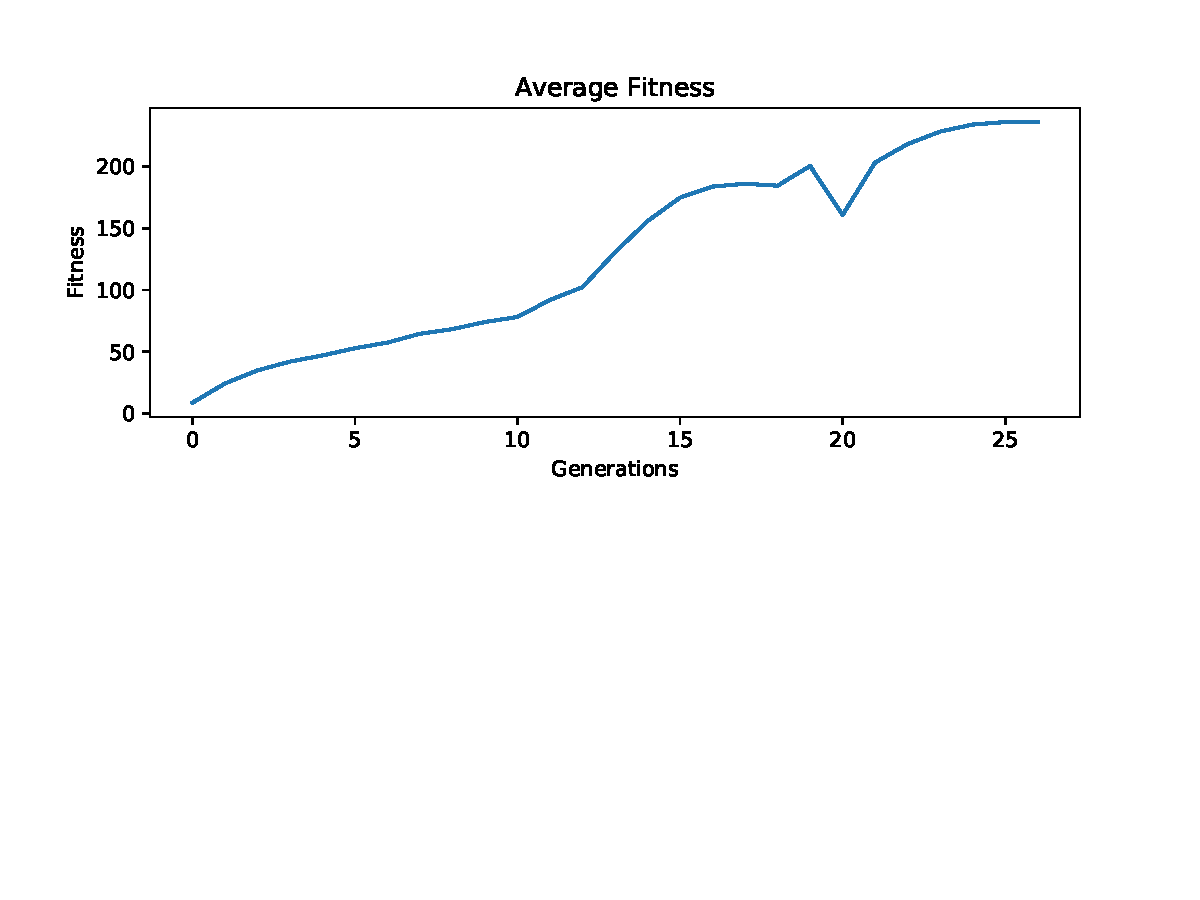
\includegraphics[scale=0.41, clip, trim=0.5cm 7.2cm 0.5cm 0.7cm]{../../NatComputingCW/function_exp_31_tree.pdf} 
\caption{Average fitness of the GP throughout the generations with extended operator function set $max(max(28 + x, max(41 + x, (max(x, 16)×(-112) + 56 \;mod\; x^2) + (-520 + max(x, 29)) mod \; x \;mod \;2\; mod\; (51 x))) + x^2, max(15 x, x \;mod \;53 \;mod\; max(11, x)) + (x - 46))$ , depth limit 5, population size 5000, birth-rate 0.7)}
\label{fig:extension_function_1}
\end{figure}

\begin{figure}[h]
\centering
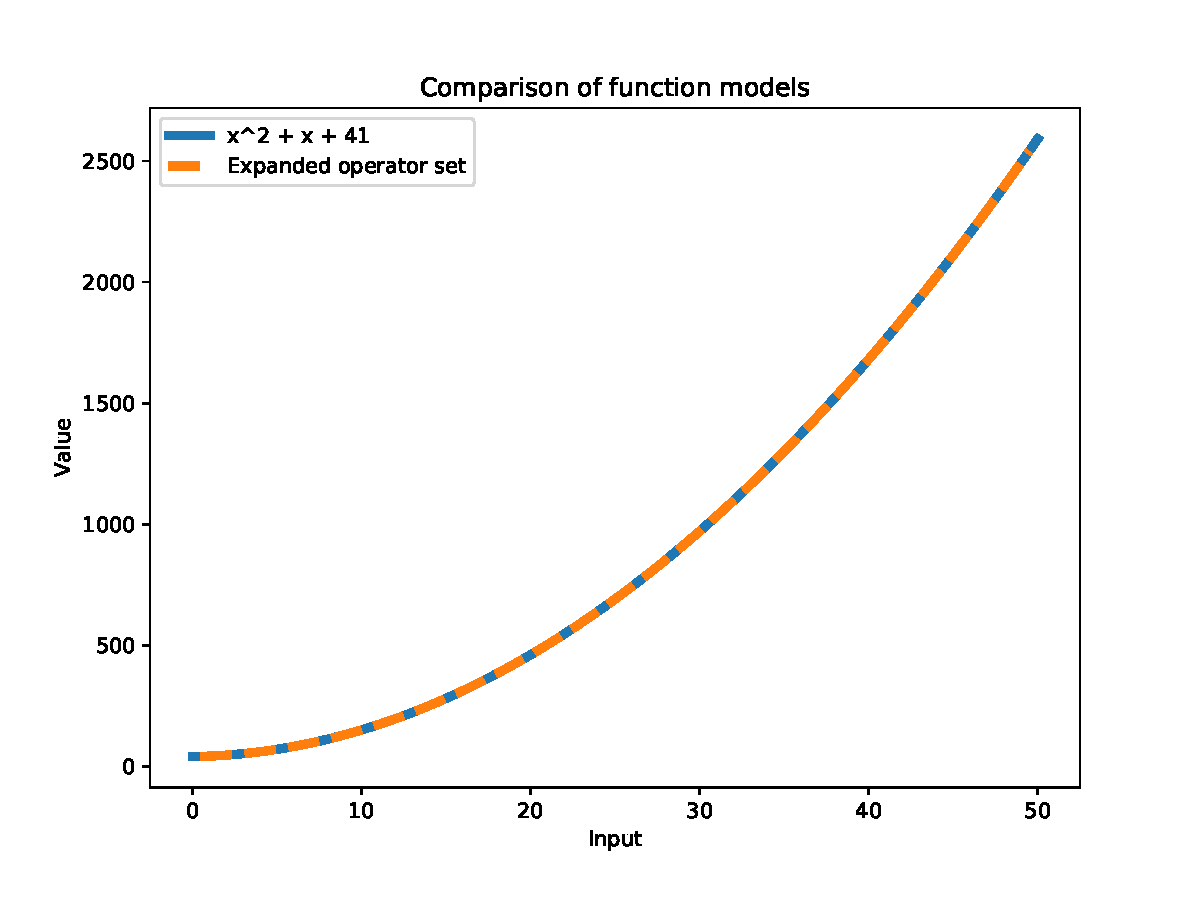
\includegraphics[scale=0.41, clip, trim=0.5cm 2.2cm 0.5cm 0.5cm]{../../NatComputingCW/extension_function.pdf} 
\caption{$x^2 + x +41$ and the GP-tree with extended operator function set $max(max(28 + x, max(41 + x, (max(x, 16)×(-112) + 56 \;mod\; x^2) + (-520 + max(x, 29)) mod \; x \; mod \;2\; mod \;(51 x))) + x^2, max(15 x, x \;mod \;53 \;mod\; max(11, x)) + (x - 46))$ over the real number interval $[0.0, 50.0]$ (mutation-rate 0.1, number of populations 1, coefficient bounds $[-61, 61]$, depth limit 5, population size 5000, birth-rate 0.7)}
\label{fig:extension_function_2}
\end{figure}

\subsection*{GP and Simulated Annealing}

\begin{algorithm}[h]
\begin{algorithmic}
   \STATE {\bfseries Input:} $p$, $iterations$, $temp$, $temp_{change}$
   \STATE $p_{current} \leftarrow p$
   \STATE $p_{best} \leftarrow p_{current}$
   \FOR{$i=1$ {\bfseries to} $iterations$}
   \STATE $p_i \leftarrow ChangeTerminals(p_{current})$
   \STATE $temp \leftarrow temp \cdot temp_{change}$
   \IF{$f(p_i) \leq f(p_{current})$} 
       \STATE $p_{current} \leftarrow p_i$
       \IF{$f(p_i) \leq f(p_{best})$} 
           \STATE $p_{best} \leftarrow p_i$
       \ENDIF
   \ELSIF {True $\sim \exp(\frac{f(p_{current})-f(p_{p_i})}{temp})$}
   	   \STATE $p_{current} \leftarrow p_i$
   \ENDIF
   \ENDFOR \\
   \textbf{return} $p_{best}$
\end{algorithmic}
  \caption{Simulated Annealing}
  \label{alg:SimAnn}
\end{algorithm}

\begin{figure}[h]
\centering
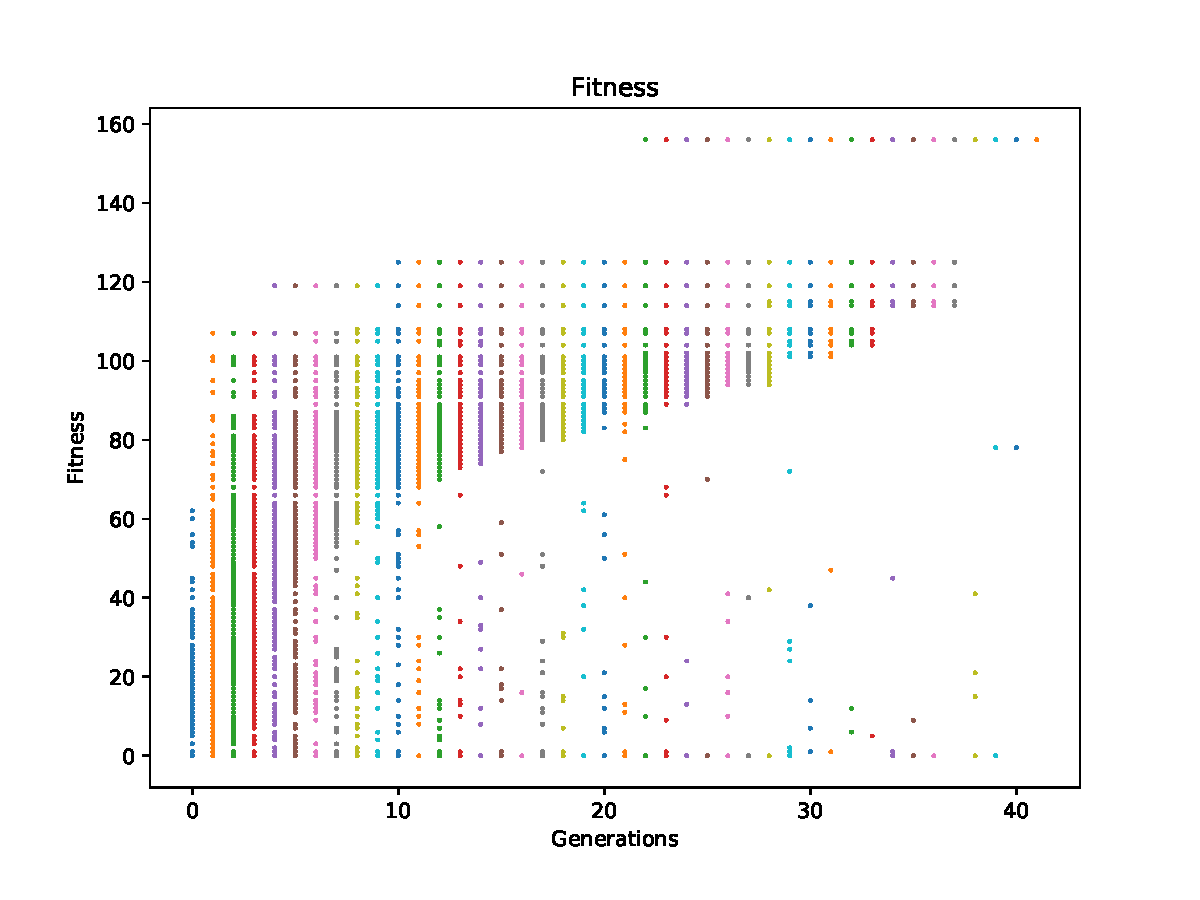
\includegraphics[scale=0.41, clip, trim=0.5cm 2.2cm 0.5cm 0.5cm]{../../NatComputingCW/Tree_simAnn_scatter.pdf} 
\caption{GP with Simulated Annealing fitness throughout the generations (iterations 700, temperature 70000, temperature change 0.98, mutation-rate 0.1, number of populations 1, coefficient bounds $[1, 42]$, depth limit 3, population size 5000, birth-rate 0.7)}
\label{fig:simAnn_1}
\end{figure}

\begin{figure}[h]
\centering
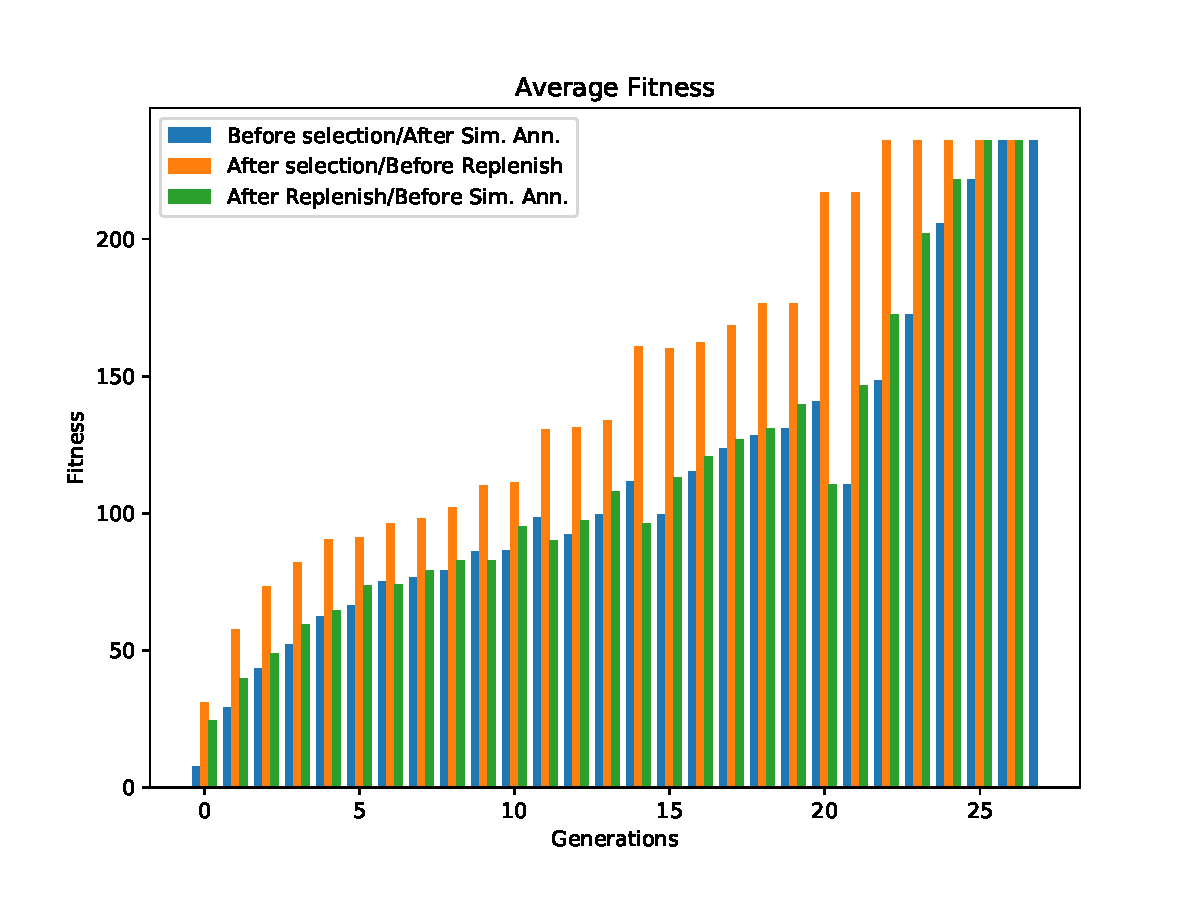
\includegraphics[scale=0.41, clip, trim=0.5cm 2.2cm 0.5cm 0.5cm]{../../NatComputingCW/Tree_simAnn_bars.pdf} 
\caption{GP with Simulated Annealing average fitness throughout the generations within the different phases (iterations 700, temperature 70000, temperature change 0.98, mutation-rate 0.1, number of populations 1, coefficient bounds $[1, 42]$, depth limit 3, population size 5000, birth-rate 0.7)}
\label{fig:simAnn_2}
\end{figure}

\end{appendices}
\end{document}